\documentclass[10pt,a4paper]{article}
\usepackage[margin=16mm]{geometry}
\usepackage[T1]{fontenc}
\usepackage{lmodern,microtype,graphicx,booktabs}
\usepackage[hidelinks,pdfauthor={},pdftitle={Computer Architecture - Technical Brief Report}]{hyperref}
\setlength{\parindent}{0pt}\setlength{\parskip}{4pt}
\begin{document}
{\LARGE\bfseries Computer architecture experiments}\par
{\large Technical Brief Report}\par
Three HY425 assignments study how branch predictors, out-of-order execution resources, and cache/prefetch policies influence simulated instruction throughput. The collection combines original C++ predictor source, completed course reports, editable workbooks, and saved gem5 statistics. The current runnable workflow reanalyzes those historical results.
\section*{Engineering scope}
\textbf{Branch prediction.} GAg uses a shared global-history register to select saturating counters in a pattern table. PAg first selects local history using the branch address, then indexes a shared counter table. The supplied source exposes lookup, counter training, outcome-history updates, and skipped wrong-path updates. The archived counter dump supports 20 predictor/benchmark comparisons. Its reported branch ratio divides committed branch mispredicts by predictor lookups. This is not automatically conditional-branch error rate or prediction accuracy.

\textbf{CPU resource tuning.} The second study varies load/store queue capacity, reorder-buffer size, and functional-unit counts. The workbook contains 25 usable rows across five benchmarks. The analysis recomputes every arithmetic mean from the five numeric cells and checks it against the stored average. The original procedure is sequential: later parameter groups retain earlier choices. The results therefore illustrate local tradeoffs rather than an exhaustive factorial optimum. The report's multiplicative MiP metric is a coursework resource proxy, not a hardware power or area measurement.

\textbf{Memory hierarchy.} Five compressed data files preserve the original statistics text for 370 runs: 12 L1 configurations, 54 L2 configurations, and eight prefetcher configurations, each evaluated on five benchmarks. The parser extracts IPC, L1D and L2 miss-rate counters separately, and DRAM bandwidth. Per-configuration summaries require exactly one result from each benchmark.
\begin{center}
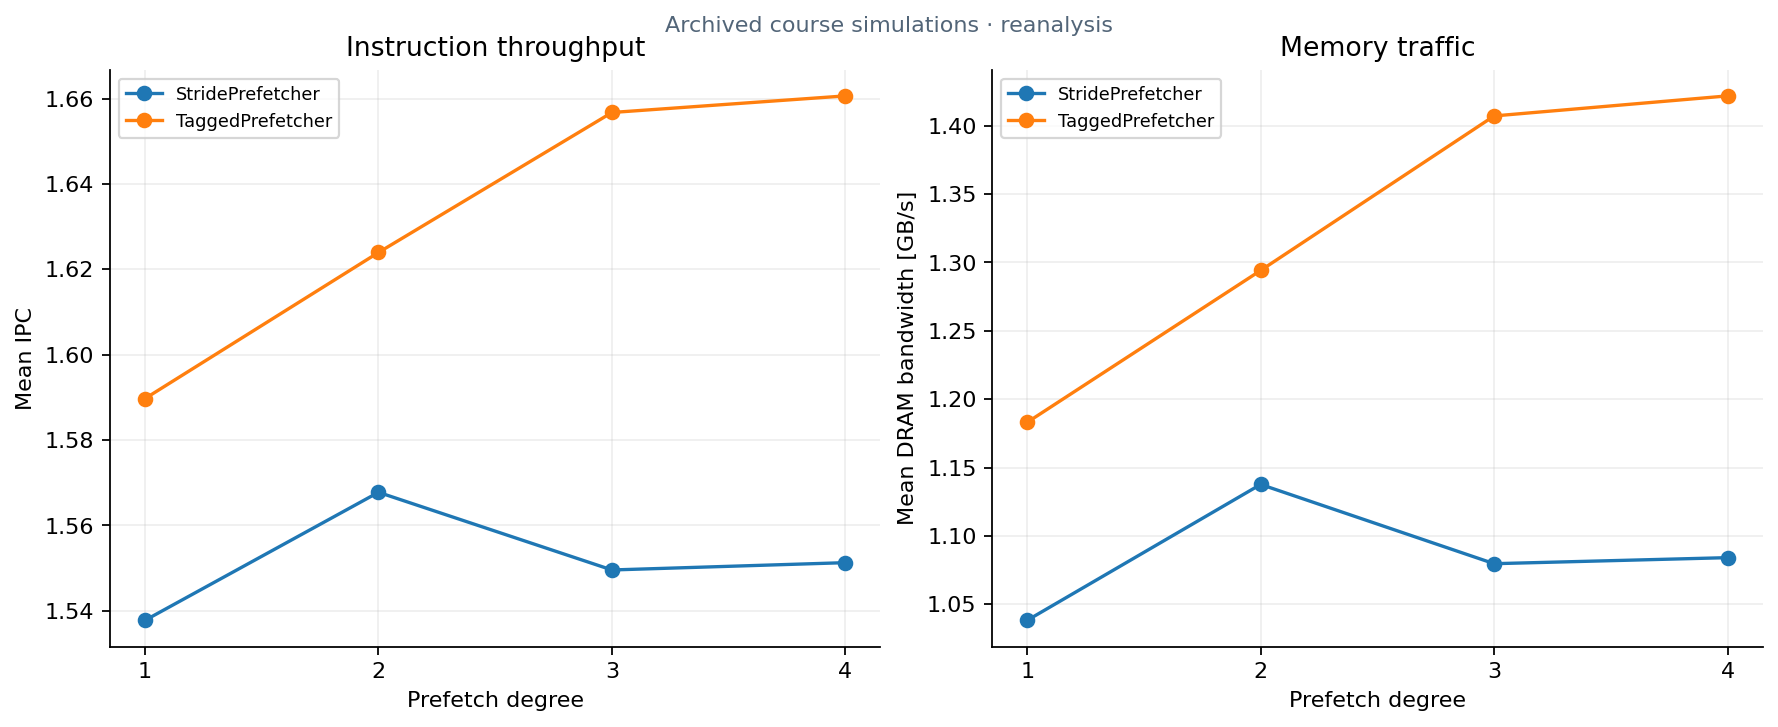
\includegraphics[width=.85\linewidth]{assets/prefetchers.png}
\end{center}
{\small Recomputed means from the saved prefetch experiments. Increased IPC and increased memory traffic are distinct outcomes. Bandwidth is decimal GB/s, derived from the original byte/second counter.}
\section*{Evidence, interpretation, and reproduction}
The 128-byte, 4-way L1 configuration has mean IPC 1.4015454 in the archived sweep. The Tagged prefetcher at degree 4 has mean IPC 1.6606342, while degree 3 reaches 1.6567462. These figures characterize the supplied five workloads, not new simulator runs or a general architectural recommendation.

Four automated checks validate final-dump parsing, branch-counter arithmetic, workbook means, complete sweep coverage, and a known L1 average. Original reports remain unchanged. Current metric names distinguish L1D from L2 miss rates and use bytes/second for DRAM bandwidth.

The course gem5 tree, parameter declarations, build registration, and benchmark programs are absent. PAg's entry-count/bit-shift mask mismatch also needs repair before integration. No fresh simulator run or predictor correctness claim is made.

Install \texttt{requirements.txt}, then run \texttt{python tools/analyze.py} and \texttt{python tools/plot\_results.py}. The \href{https://github.com/mitsosasim/computer_architecture/blob/main/docs/SETUP.md}{setup guide} covers reproduction and metric definitions. Original coursework identifies Dimitris Asimakopoulos, csd4845.
\end{document}
